\documentclass[tikz,border=10pt]{standalone}
\usepackage{tikz}
\usetikzlibrary{shapes.geometric, arrows.meta, positioning, fit, backgrounds, shapes.misc}

\begin{document}
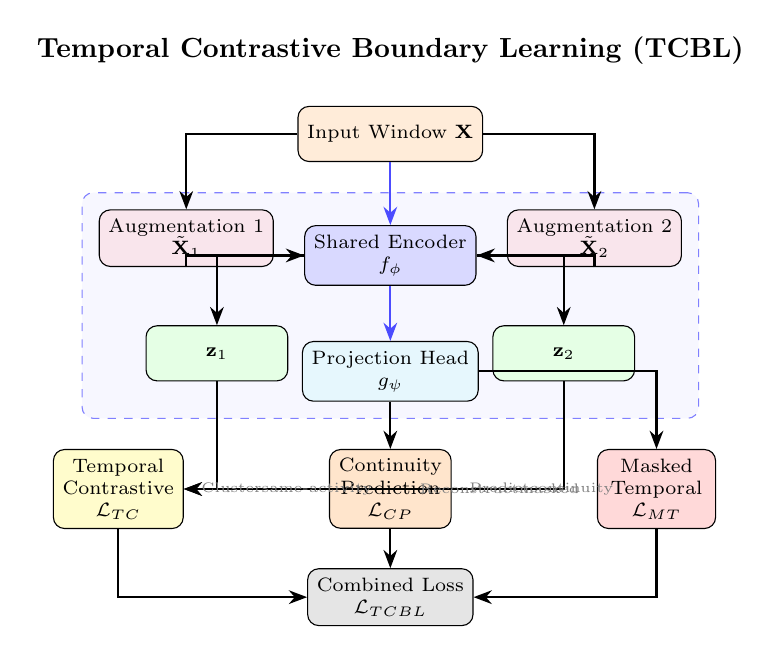
\begin{tikzpicture}[
    node distance=0.5cm and 0.7cm,
    block/.style={rectangle, draw, fill=blue!10, rounded corners, 
        minimum height=0.7cm, minimum width=1.8cm, align=center, font=\scriptsize},
    lossblock/.style={rectangle, draw, fill=red!10, rounded corners,
        minimum height=0.6cm, minimum width=1.5cm, align=center, font=\scriptsize},
    arrow/.style={-Stealth, thick},
    dataarrow/.style={-Stealth, thick, blue!70}
]

% Title
\node[font=\bfseries] (title) {Temporal Contrastive Boundary Learning (TCBL)};

% Input
\node[block, fill=orange!15, below=0.4cm of title] (input) {Input Window $\mathbf{X}$};

% Augmentation branch
\node[block, fill=purple!10, below left=0.6cm and 0.3cm of input] (aug1) {Augmentation 1\\$\tilde{\mathbf{X}}_1$};
\node[block, fill=purple!10, below right=0.6cm and 0.3cm of input] (aug2) {Augmentation 2\\$\tilde{\mathbf{X}}_2$};

% Shared encoder
\node[block, fill=blue!15, below=0.8cm of input] (encoder) {Shared Encoder\\$f_\phi$};

% Features
\node[block, fill=green!10, below left=0.5cm and 0.2cm of encoder] (z1) {$\mathbf{z}_1$};
\node[block, fill=green!10, below right=0.5cm and 0.2cm of encoder] (z2) {$\mathbf{z}_2$};

% Projection head
\node[block, fill=cyan!10, below=0.7cm of encoder] (proj) {Projection Head\\$g_\psi$};

% Three pretext tasks
\node[lossblock, fill=yellow!20, below left=0.6cm and 1.5cm of proj] (tc) {Temporal\\Contrastive\\$\mathcal{L}_{TC}$};
\node[lossblock, fill=orange!20, below=0.6cm of proj] (cp) {Continuity\\Prediction\\$\mathcal{L}_{CP}$};
\node[lossblock, fill=red!15, below right=0.6cm and 1.5cm of proj] (mt) {Masked\\Temporal\\$\mathcal{L}_{MT}$};

% Combined loss
\node[lossblock, fill=gray!20, below=0.5cm of cp] (total) {Combined Loss\\$\mathcal{L}_{TCBL}$};

% Arrows
\draw[dataarrow] (input) -- (encoder);
\draw[arrow] (input) -| (aug1);
\draw[arrow] (input) -| (aug2);
\draw[arrow] (aug1) |- (encoder);
\draw[arrow] (aug2) |- (encoder);
\draw[dataarrow] (encoder) -- (proj);
\draw[arrow] (encoder) -| (z1);
\draw[arrow] (encoder) -| (z2);
\draw[arrow] (proj) -- (cp);
\draw[arrow] (z1) |- (tc);
\draw[arrow] (z2) |- (tc);
\draw[arrow] (proj) -| (mt);
\draw[arrow] (tc) |- (total);
\draw[arrow] (cp) -- (total);
\draw[arrow] (mt) |- (total);

% Annotations
\node[font=\tiny, right=0.1cm of tc, text=gray] {Cluster\\same-activity};
\node[font=\tiny, right=0.1cm of cp, text=gray] {Predict\\continuity};
\node[font=\tiny, left=0.1cm of mt, text=gray] {Reconstruct\\masked};

% Background
\begin{scope}[on background layer]
    \node[fit=(aug1)(aug2)(encoder)(z1)(z2)(proj), 
          draw=blue!50, dashed, rounded corners, 
          fill=blue!3, inner sep=6pt] {};
\end{scope}

\end{tikzpicture}
\end{document}
